%% ===========================================================================
%% Information Processing & Management — ANONYMIZED MANUSCRIPT (double-blind)
%% Compile with pdflatex (figures are PDF in ./paper_figures/).
%% Author identities, affiliations, acknowledgements, and CRediT are in the
%% SEPARATE title_page.tex file (do NOT include them here — double-anonymized review).
%% ===========================================================================
\documentclass[preprint,12pt]{elsarticle}

\usepackage{amssymb}
\usepackage{amsmath}
\usepackage{booktabs}   % horizontal rules only (no vertical rules / shading) per IP&M
\usepackage{graphicx}   % also loaded by elsarticle.cls
\usepackage{url}

\journal{Information Processing \& Management}

\begin{document}

\begin{frontmatter}

\title{Popularity Bias and Cold-Start in Patent Technology-Transfer
Demand Prediction: A Diagnostic Evaluation}
%% Alternative title (also IP&M-appropriate, slightly shorter):
%% \title{When Learned Models Do Not Beat a Popularity Baseline:
%% A Diagnostic Evaluation of Patent Technology-Transfer Demand Prediction
%% under a Temporal, Hard-Negative Protocol}

%% --- Author block intentionally omitted for double-anonymized review. ---
%% (Authors, affiliations, corresponding-author details, acknowledgements,
%%  and CRediT statements are provided in title_page.tex.)

\begin{abstract}
Predicting which company will acquire the rights to a given patent --- patent
technology-transfer demand prediction --- can be framed as link prediction on a
heterogeneous graph coupling a patent--cites--patent network with
patent--transfer--company edges. We evaluate this task on the Korean KIPRIS
dataset (370,666 patents; 122,519 companies) under a realistic protocol: transfer
edges are split temporally by registration date, candidates are same-IPC hard
negatives, and ties are resolved by average rank. Under this protocol every
learned model we test --- heterogeneous GNNs (GraphSAGE, GAT), collaborative
filtering (LightGCN, NGCF), matrix factorization (SVD), structural heuristics
(Common Neighbors, Adamic--Adar), and a text MLP --- falls below a simple
most-popular baseline (MostPop NDCG@10\,=\,0.197; the strongest learned model, a
text MLP, reaches only 0.150), with AUC near chance (0.42--0.60). Two causes
account for this: popularity bias (98.8\% of GraphSAGE and 57.8\% of GAT errors
are losses to a more-popular hard negative, and learned-model scores track
popularity up to $\rho=0.96$)
and patent cold-start (91.7\% of test patents unseen; SVD
NDCG@10\,=\,0.000 on new patents). We document an evaluation artifact whereby a
strict greater-than tie-break inflates degenerate cold-start models toward
high scores, which average-rank tie-breaking removes. A controlled random-split
contrast shows the protocol determines the outcome: a random split lowers cold-start to 2.4\%
and makes SVD the single best method (NDCG@10\,=\,0.442, AUC\,=\,0.830), the reversal
of the temporal verdict. We contribute the evaluation protocol, a suite of bias and cold-start
diagnostics, and a symmetric grid of mitigation baselines that yield only
partial, unstable gains.
\end{abstract}

\begin{highlights}
\item Under a temporal, same-IPC hard-negative protocol, no learned model beats a popularity baseline on KIPRIS patent-transfer prediction.
\item The failure is traced to popularity bias (score--popularity $\rho$ up to 1.0) and a 91.7\% patent cold-start regime.
\item A strict tie-break inflates degenerate cold-start models to near-perfect scores; average-rank tie-breaking is required.
\item A random split reverses the verdict (SVD becomes best at 0.442), showing that the protocol, not the model, determines the outcome.
\item Standard popularity-bias mitigations (IPS, logQ, debiased sampling) give only partial, unstable gains.
\end{highlights}

\begin{keyword}
patent technology transfer \sep link prediction \sep graph neural networks \sep
popularity bias \sep cold-start \sep evaluation methodology
\end{keyword}

\end{frontmatter}

%% ===========================================================================
\section{Introduction}
\label{sec:intro}

Patent technology transfer --- the licensing, assignment, or sale of patent rights
from one party to another --- is a central mechanism by which research output is
converted into commercial use. For technology-holding institutions and the
intermediaries that support commercialization, a recurring operational question
is: \emph{given a particular patent, which companies are plausible recipients of
its rights?} Answering it well would shorten the search for licensees and help
allocate scarce brokerage effort \cite{kimgeum2020,lee2016}. In the Korean setting,
where public technology-transfer programs and the KIPRIS registry make large-scale
transaction records observable, the question is both economically meaningful and
empirically tractable \cite{rhee2026,parkyoon2017}. We refer to this task as
\emph{technology-transfer demand prediction}, with the explicit caveat that the
available supervision is realized transfers rather than latent demand.

The task has a natural relational structure. Patents cite other patents and the
scientific literature --- reference signals rich enough to have motivated dedicated
large-scale extraction pipelines \cite{abbasiantaeb2025} --- patents are transferred
to companies, and companies accumulate portfolios. This induces a heterogeneous
graph with \emph{patent} and \emph{company} nodes and two edge types
(patent--cites--patent and patent--transfer--company), in which demand prediction
becomes link prediction. Cast this way, the problem invites graph representation
learning and collaborative filtering: GNNs such as GraphSAGE \cite{hamilton2017}
and graph attention networks \cite{velickovic2018,brody2022}, CF models such as NGCF
\cite{wang2019} and LightGCN \cite{he2020}, and matrix factorization \cite{rendle2009},
with patent text encoded by sentence embeddings \cite{reimers2019} providing node
features. The expectation that such methods outperform simple heuristics is the
default working hypothesis in much of the literature and motivates a growing line of
patent-recommendation systems \cite{krestel2021,choi2019,chendeng2023,liu2024}. Most
directly, a recent GAT--NGCF firm--patent recommender on Korean technology-transfer
data reports Recall@5\,=\,0.998 and NDCG@5\,=\,0.997 \cite{kim2025}. Such
near-perfect figures rest on random-split, sampled-negative evaluation; the
gap we document is that they do not survive a leakage-free, temporal, same-IPC
hard-negative re-evaluation, which is the research gap this paper addresses.

That expectation is sensitive to how performance is measured. \emph{Random edge
splits} break temporal order and leak future transfers \cite{meng2020};
\emph{uniform random negatives} make ranking easy and inflate AUC relative to a
deployment setting where all candidates are topically relevant \cite{krichene2020};
and headline AUC can mask the popularity bias known to dominate recommendation under
skewed exposure \cite{abdollahpouri2019,steck2018,zhu2021,boratto2021} --- a bias
whose effect on accuracy and fairness is itself a function of dataset characteristics
\cite{deldjoo2021}, and whose corrective methods transfer only partially to practice
\cite{boratto2023}. A realistic protocol must therefore combine temporal ordering,
same-class hard negatives, explicit cold-start accounting, and care over tie-breaking.

In this paper we evaluate the task under such a protocol and report a primarily
diagnostic finding: under a temporal 70/15/15 split with same-IPC hard negatives
($n_{\mathrm{neg}}=100$) and an average-rank tie-break, \emph{every learned model we
test falls below simple popularity baselines.} The dataset comprises 370,666
patents, 122,519 companies, and $\approx$910,000 citation edges, yielding
$\approx$220,284 temporally held-out test queries. A most-popular ranker attains
NDCG@10\,=\,0.197; an IPC-conditional skyline reaches 0.199 (the top NDCG@10, though
at a below-chance global AUC of 0.416; see \S\ref{sec:main}); and NGCF --- which our
diagnostics show to be a popularity ranker ($\rho=0.96$) --- reaches 0.196. The
strongest learned model with above-chance discrimination is a text MLP at 0.150;
among graph models, GraphSAGE+logQ reaches 0.125 and GAT+logQ 0.107; all lie well
below the popularity baselines, and the AUC of every model is near or below chance
(0.42--0.60). The pattern holds across GNNs, CF, MF, structural heuristics, and a
text MLP. It mirrors a broader concern that learned recommenders often fail to beat
well-tuned baselines \cite{dacrema2019} and that easy negatives inflate GNN
link-prediction \cite{li2023}.

We trace the result to two causes and quantify each. First, \emph{popularity bias}:
98.8\% of GraphSAGE and 57.8\% of GAT errors are losses to a more-popular same-IPC
hard negative; the hard-negative inversion rate (the share of queries in which a more-popular candidate outranks the positive) is 56\% for MostPop and NGCF and 28\%
for GAT; and score--popularity Spearman correlation is 1.0 for MostPop and 0.96 for
NGCF. A GAT attention analysis (Mann--Whitney U over hub vs.\ non-hub edges,
$p=1.0$) shows no down-weighting of popular hubs. Second, \emph{extreme patent
cold-start}: 91.7\% of test patents are unseen in training, and SVD collapses to
NDCG@10\,=\,0.000 on new patents. We then test whether popularity-bias mitigations
recover learned models above the baselines; across more than 20 configurations the
gains are partial and unstable (\S\ref{sec:mitigation}).

A further contribution is methodological. Under a strict greater-than tie-break,
cold-start models whose scores are degenerate place the positive first among tied
candidates and attain inflated scores (\S\ref{sec:tiebreak}); an average-rank
tie-break removes this artifact. These observations motivate three research
questions addressed in the paper:
\begin{itemize}
\item \textbf{RQ1.} Does a realistic protocol (temporal split + same-IPC hard
negatives) change measured performance relative to a random split?
(\S\ref{sec:rq1}: yes.)
\item \textbf{RQ2.} What accounts for the performance --- popularity bias, cold-start,
or both --- and how is each quantified? (\S\ref{sec:popbias}--\S\ref{sec:error}.)
\item \textbf{RQ3.} Can popularity-bias mitigations recover learned models above the
popularity baselines? (\S\ref{sec:mitigation}: not reliably.)
\end{itemize}

\noindent The contributions are: (i) a leakage-free evaluation protocol for the
task on KIPRIS, combining a temporal split, same-IPC hard negatives, explicit
cold-start accounting, and an average-rank tie-break; (ii) a diagnosis that
GNNs, CF, MF, structural heuristics, and a text MLP all fall below popularity
baselines, with AUC near chance, together with the quantification of
popularity bias and cold-start that explains why; (iii) a reusable suite of
bias-diagnostic tools that localize the failure; (iv) a mitigation grid showing
only partial, unstable gains; and (v) identification of a strict-tie-break
artifact and its average-rank correction, corroborated by an unsampled
full-pool metric and a temporal-versus-random contrast. The aim is not a
winning model but an evaluation protocol and diagnosis to discipline future
work. Figure~\ref{fig:overview} gives an overview.

\begin{figure*}[t]
\centering
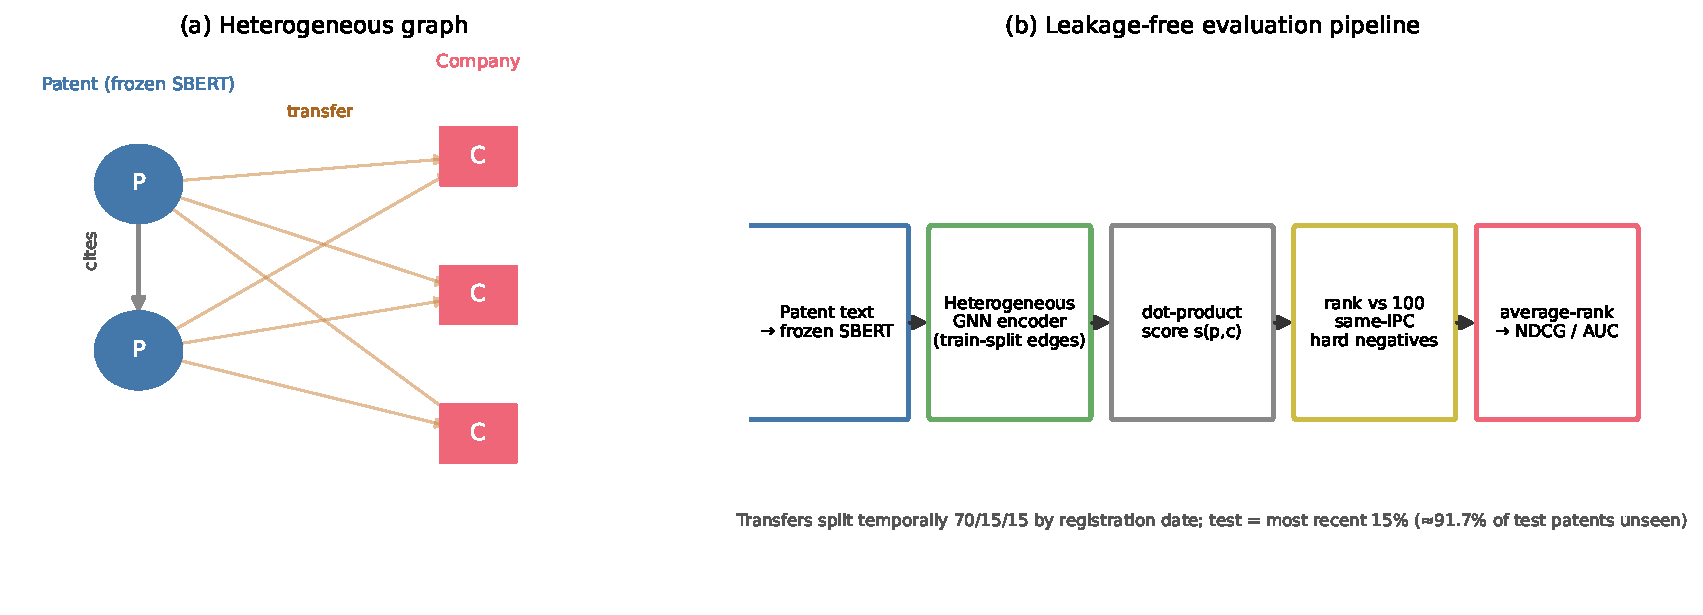
\includegraphics[width=0.92\textwidth]{paper_figures/Figure_1}
\caption{Overview of the task and the central finding. We frame patent
technology-transfer demand prediction as link prediction on a heterogeneous
patent--citation--transfer graph and evaluate it under a leakage-free protocol
(temporal split; encoding on training-split edges only; ranking the true acquirer
against 100 same-IPC hard negatives; average-rank tie-break). Under this protocol
every learned model falls below a most-popular baseline and discriminates near
chance, which we trace to popularity bias and an extreme (91.7\%) patent cold-start
regime; a conventional random split would reverse this verdict.}
\label{fig:overview}
\end{figure*}

%% ===========================================================================
\section{Related Work}
\label{sec:related}

Our study sits at the intersection of four lines of work: patent analytics and
technology-transfer prediction; GNNs for link prediction and recommendation;
popularity bias and debiasing; and evaluation methodology for ranking under temporal
and sampled-metric constraints. We also use structural link-prediction heuristics as
non-learned baselines. The recurring theme is that this paper's contribution is diagnostic:
we do not propose a model that outperforms prior art, but an evaluation protocol and
diagnostic tools that explain \emph{why}, on this task and dataset, learned models do
not separate from popularity baselines.

\subsection{Patent Analytics and Technology-Transfer Prediction}
A substantial body of work uses patent metadata, classification codes, and citation
networks --- including recent work on extracting and matching patent in-text
references at scale \cite{abbasiantaeb2025} --- to characterize technological
trajectories and forecast emerging technologies \cite{krestel2021,erdi2013}. Within
this literature, technology transfer has been examined as a prediction target
\cite{kimgeum2020,rhee2026}, with approaches ranging from feature-engineered and BERT
classifiers \cite{kimgeum2020} to collaborative filtering over IPC/portfolio
structure \cite{parkyoon2017,lee2016} and graph formulations
\cite{kim2025,chendeng2023,liu2024}. Several graph recommenders report near-perfect
retrieval (e.g., Recall@5\,=\,0.998 \cite{kim2025}) under random-split, sampled-negative
evaluation --- precisely the regime our protocol revisits. Three properties
distinguish our setting: the supervision is a \emph{realized} transfer; the
prediction is prospective; and the patent side is severely cold-start (91.7\% of test
patents are new). Table~\ref{tab:protocol} contrasts the evaluation safeguards our
protocol applies with those prevailing in prior graph-based patent recommenders.

\begin{table}[t]
\centering
\caption{Evaluation safeguards in the protocol of this paper versus those typically
applied in prior graph-based patent-recommendation studies (e.g.,
\cite{kim2025,chendeng2023,liu2024}). ``Typical'' denotes the prevailing practice, not
any single paper. Each safeguard counters a specific source of optimism (future
leakage, easy negatives, tie degeneracy, an absent skyline, hidden cold-start, or a
single arbitrary cutoff).}
\label{tab:protocol}
\begin{tabular}{lcc}
\toprule
Evaluation safeguard & Typical prior eval & This work \\
\midrule
Temporal (forward-in-time) split            & usually random   & yes \\
Hard negatives from the same IPC class       & uniform / in-batch & yes \\
Average-rank tie-break                        & unspecified      & yes \\
Popularity skyline as the bar to beat         & weak / absent    & yes \\
Cold-start fraction reported and decomposed   & rarely           & yes \\
AUC reported beside top-$K$                    & top-$K$ only     & yes \\
Unsampled full-IPC-pool metric                & no               & yes \\
Rolling-origin (multiple temporal cutoffs)     & no               & yes \\
Multi-seed, paired tests, multiplicity control & rare             & yes \\
\bottomrule
\end{tabular}
\end{table}

\subsection{GNNs for Link Prediction and Recommendation}
GraphSAGE \cite{hamilton2017} introduced inductive aggregation; GAT \cite{velickovic2018}
learned attention weights, and GATv2 \cite{brody2022} corrected a static-attention
limitation. In recommendation, LightGCN \cite{he2020} simplified propagation, whereas
NGCF \cite{wang2019} retains feature transformation; DropEdge \cite{rong2020} is a
structural regularizer. Heterogeneous/relational variants such as R-GCN
\cite{schlichtkrull2018} and the Heterogeneous Graph Transformer \cite{hu2020hgt}
extend message passing to typed graphs; SEAL \cite{zhang2018} frames link prediction
as subgraph classification. We adopt these architectures essentially as published and
ask whether, under a leakage-free temporal split with same-IPC hard negatives, they
separate from non-learned baselines. They do not; \S\ref{sec:popbias} examines why.

\subsection{Popularity Bias and Debiasing}
A well-documented failure mode of implicit-feedback recommenders is popularity bias:
models score frequently interacted items highly regardless of relevance, and standard
metrics reward this \cite{abdollahpouri2019,steck2018}. IPS methods reweight by inverse
exposure probability \cite{schnabel2016,saito2020}; sampling-bias-corrected training
(logQ) adjusts sampled-softmax logits by log-frequency \cite{yi2019}; and the BPR
framework \cite{rendle2009} underlies much of this work. Within the present venue, a
line of work has examined this bias directly: Boratto et al.\ \cite{boratto2021}
connect user- and item-side perspectives on popularity debiasing; Deldjoo et al.\
\cite{deldjoo2021} show the accuracy/fairness consequences are governed by dataset
characteristics; and Boratto et al.\ \cite{boratto2023} report that consumer-fairness
mitigations transfer only partially to practice --- a partial-and-unstable pattern
matching our own results. Popularity bias is the central finding of our diagnosis,
made explicit rather than assumed (\S\ref{sec:popbias}).

\subsection{Evaluation Methodology}
Offline recommender evaluation is fragile: many neural recommenders fail to beat
tuned baselines \cite{dacrema2019,rendle2019}; sampled top-$K$ metrics can be
inconsistent with full ranking \cite{krichene2020,canamares2020,ihemelandu2023};
random splits leak future information relative to temporal splits
\cite{meng2020,ji2023}; and easy negatives inflate GNN link prediction \cite{li2023}.
Hidasi and Czapp \cite{hidasi2023} catalogue widespread offline-evaluation flaws,
including degeneracies of the kind our tie-break artifact exemplifies. Our protocol
operationalizes these recommendations and adds an average-rank tie-break necessary to
avoid inflating no-information cold-start models.

\subsection{Structural Heuristics and Cold-Start}
Common Neighbors and Adamic--Adar are strong, parameter-free baselines for
homogeneous link prediction. Cold-start, where items carry no interaction history,
is addressed by content- and meta-learning methods \cite{volkovs2017}; our setting is
an extreme instance (91.7\% new patents). We include Common Neighbors and
Adamic--Adar over the citation graph; both fall below the popularity skylines
(NDCG@10\,=\,0.065--0.066), confirming that citation-structure overlap alone does not
recover the transfer signal.

%% ===========================================================================
\section{Dataset, Heterogeneous Graph, and Models}
\label{sec:data}

\subsection{Data}
The KIPRIS patent data is obtained from the Korea Intellectual Property Rights
Information Service API. We use three tables: \texttt{patents} (application number,
IPC code, title, abstract), \texttt{transfers} (application number, acquiring
company, registration date), and \texttt{citings} (citing/cited application numbers).
Application numbers are cleaned to digits only before joining. The corpus contains
370,666 patents, 122,519 companies, and $\approx$910,000 citation edges. Patent text
(title + abstract) is encoded once with a frozen multilingual Sentence-BERT model
(\texttt{paraphrase-multilingual-MiniLM-L12-v2}) \cite{reimers2019,reimers2020} into
384-dimensional features, row-aligned to the patent table.

\subsection{Heterogeneous Graph and Problem Formulation}
We model the task as link prediction on a heterogeneous graph $G=(V,E)$ with
$V=P\cup C$ ($P$ patents, $C$ companies) and two undirected-typed edge sets:
citations $E_{\mathrm{cite}}\subseteq P\times P$ and realized transfers
$E_{\mathrm{tr}}\subseteq P\times C$. Each patent carries its frozen 384-d SBERT
feature $x_p$. For the GNN encoders each company is assigned a \emph{fixed-random}
feature $x_c\in\mathbb{R}^{64}$ (drawn once as $\mathcal{N}(0,0.1^2)$, never updated),
with the only learned company-side parameters being a shared linear projection; only
LightGCN/NGCF use a learnable per-company identity embedding ($d=64$). We ablate this
random-feature choice with a leakage-free content company representation in
\S\ref{sec:content}. An encoder
$f_\theta$ maps nodes to $h_p,h_c\in\mathbb{R}^{16}$ by message passing over
$E_{\mathrm{cite}}$ and the \emph{training-split} transfers only, and a parameter-free
decoder scores a pair by the dot product $s(p,c)=h_p^{\top}h_c$; this is the same
score optimized by the training loss (\S\ref{sec:models}) and re-ranked by the
IPS / logQ mitigations (\S\ref{sec:mitigation}). For a held-out test transfer
$(p,c^{+})$ we form $\mathrm{Cand}(p)=\{c^{+}\}\cup C^{-}(p)$, where $C^{-}(p)$ are
$n_{\mathrm{neg}}=100$ same-IPC hard negatives --- companies that received a same-IPC
patent in training but not $p$ --- and report the average rank of $c^{+}$.
Table~\ref{tab:notation} summarizes the notation. A construct-validity caveat
underlies the study: the supervision is \emph{realized} transfers, so a model that
perfectly predicted them would recover the historical (and biased) matching process,
not latent demand.

\begin{table}[t]
\centering
\caption{Notation.}
\label{tab:notation}
\begin{tabular}{ll}
\toprule
Symbol & Meaning \\
\midrule
$G=(V,E)$, $V=P\cup C$ & heterogeneous graph; patent / company nodes \\
$E_{\mathrm{cite}}, E_{\mathrm{tr}}$ & citation edges; realized transfer edges \\
$x_p\in\mathbb{R}^{384}$, $x_c\in\mathbb{R}^{64}$ & frozen SBERT patent / company feature \\
$h_p,h_c\in\mathbb{R}^{16}$ & encoder node representations \\
$s(p,c)=h_p^{\top}h_c$ & dot-product link score \\
$C^{-}(p)$, $n_{\mathrm{neg}}$ & same-IPC hard negatives; candidate size (100) \\
$\mathrm{rank}(c^{+}\mid p)$ & average rank of the positive among candidates \\
\bottomrule
\end{tabular}
\end{table}

\subsection{Models Evaluated}
\label{sec:models}
We evaluate nine base models: three non-learning skylines (MostPop,
IPC-conditional MostPop-IPC, and Recency, which ranks candidate companies by the
recency of their most recent training transfer); two structural heuristics
(Common Neighbors, Adamic--Adar); SVD ($k{=}64$); a
text-only MLP; and two CF models (LightGCN, NGCF);
together with two heterogeneous GNNs (GraphSAGE, GAT), and a
\emph{symmetric mitigation grid} applying each of \{Debias, logQ, DropEdge, time
encoding, IPS\} and two stacked combinations (Debias+IPS, Time+IPS) to \emph{both}
GNN backbones. GAT uses a single-head, scatter-based attention layer that can return
attention weights for diagnostics. Training minimizes a binary cross-entropy loss
on the dot-product scores $s(p,c)=h_p^{\top}h_c$ of observed transfers (label 1)
and sampled negatives (label 0), i.e.\ $\mathcal{L}=-\sum_{(p,c^{+})}\log\sigma(s(p,c^{+}))-\sum_{(p,c^{-})}\log(1-\sigma(s(p,c^{-})))$, with early stopping on validation NDCG@10
(patience 5).

%% ===========================================================================
\section{Evaluation Protocol}
\label{sec:protocol}

\paragraph{Temporal split.} Transfers are sorted by registration date and split
70/15/15 into train/validation/test. The encoder message-passes only on training
transfers; popularity, recency, and time features are computed from the training
split alone, removing the target leakage a random split would introduce.

\paragraph{Same-IPC hard negatives.} For each test query $(p,c^{+},\mathrm{ipc4})$,
the candidate set is the positive plus $n_{\mathrm{neg}}=100$ companies drawn
(seed-fixed) from those that received a same-IPC patent in training but not $p$
(average padding rate 1.07\% when fewer than 100 same-IPC companies exist; padding fills the candidate set with uniformly drawn non-positive companies so every query has exactly $n_{\mathrm{neg}}$ negatives).

\paragraph{Metrics and tie-break.} We report Hits@$K$ and NDCG@$K$ for
$K\in\{1,3,5,10\}$, MRR, and a tie-aware rank-AUC (ties counted as 0.5). Ties are
resolved by \emph{average rank}: a candidate that ties the positive contributes 0.5
to its rank. This is necessary, because under a strict greater-than rule a no-information
model whose candidates all tie places the positive first and scores
spuriously high (\S\ref{sec:tiebreak}).

\paragraph{Statistics.} Every configuration is run over ten seeds. We test a
pre-registered family of pairwise comparisons with the Wilcoxon signed-rank test
(primary) and paired $t$-test (secondary), correcting jointly with Holm--Bonferroni,
and report percentile bootstrap 95\% confidence intervals over the $\approx$220k test
queries.

\paragraph{Reproducibility.} Seeds (torch, numpy) are fixed per run. The full
ten-seed run completes in $\approx$70 minutes on a single NVIDIA Tesla T4 and,
comparably, on Apple-Silicon CPU; LightGCN/NGCF use sparse operations unsupported by
Apple MPS, so the intended device is CUDA or CPU. We release the preprocessing and
evaluation code and a script to regenerate the SBERT embeddings.

%% ===========================================================================
\section{Results and Diagnosis}
\label{sec:results}

\subsection{Main Results}
\label{sec:main}
Table~\ref{tab:main} reports the main ten-seed results. \emph{No learned model
surpasses a simple popularity baseline.} The top three configurations are non-learned
or popularity-equivalent: MostPop-IPC (0.199), MostPop (0.197), and NGCF (0.196),
which our diagnostics (\S\ref{sec:popbias}) show to be a popularity ranker. The
strongest learned model with above-chance discrimination is the text MLP (0.150); the
best graph model is GraphSAGE+logQ (0.125), and GAT+logQ reaches 0.107 --- all below
the popularity baselines. (The IPS-penalized variants reach 0.157--0.158, but only by
driving AUC below chance; \S\ref{sec:mitigation}.) SVD (0.037), the structural
heuristics (0.065--0.066), LightGCN (0.058), and both bare GNNs (GraphSAGE 0.084, GAT
0.074) are far below. The AUC of every model lies between 0.42 and 0.60 --- near or
below chance --- confirming that none globally separates true transfers from same-IPC
alternatives. Figure~\ref{fig:main} plots all models.

\begin{table}[t]
\centering
\caption{Main results, temporal split, 10 seeds (mean). The three top NDCG@10 rows
are non-learned or popularity-equivalent. MostPop-IPC tops NDCG@10 (0.199) yet has a
below-chance AUC (0.416): ranking by same-IPC-conditional popularity places the
positive well within the top-$K$ of its own IPC class, but inverts the global
pairwise ordering of positives against out-of-class candidates, so the two metrics
diverge. Full 25-row table (with standard
deviations and all mitigation variants) in the supplementary results file.}
\label{tab:main}
\begin{tabular}{lccccc}
\toprule
Model & Hits@1 & Hits@10 & MRR & NDCG@10 & AUC \\
\midrule
MostPop                & 0.110 & 0.302 & 0.182 & 0.197 & 0.583 \\
MostPop-IPC            & 0.122 & 0.289 & 0.184 & 0.199 & 0.416 \\
Recency                & 0.029 & 0.282 & 0.128 & 0.149 & 0.602 \\
Common Neighbors       & 0.056 & 0.070 & 0.082 & 0.065 & 0.534 \\
Adamic--Adar           & 0.057 & 0.070 & 0.082 & 0.066 & 0.534 \\
SVD                    & 0.030 & 0.044 & 0.053 & 0.037 & 0.520 \\
MLP (text)             & 0.082 & 0.234 & 0.142 & 0.150 & 0.574 \\
LightGCN               & 0.019 & 0.115 & 0.063 & 0.058 & 0.509 \\
NGCF                   & 0.110 & 0.301 & 0.182 & 0.196 & 0.584 \\
GraphSAGE              & 0.042 & 0.141 & 0.087 & 0.084 & 0.473 \\
GAT                    & 0.052 & 0.102 & 0.085 & 0.074 & 0.519 \\
GAT + logQ             & 0.094 & 0.127 & 0.121 & 0.107 & 0.548 \\
GraphSAGE + logQ       & 0.099 & 0.162 & 0.133 & 0.125 & 0.540 \\
GAT + IPS              & 0.143 & 0.181 & 0.166 & 0.157 & 0.417 \\
GraphSAGE + Debias+IPS & 0.145 & 0.179 & 0.167 & 0.158 & 0.417 \\
\bottomrule
\end{tabular}
\end{table}

\begin{figure}[t]
\centering
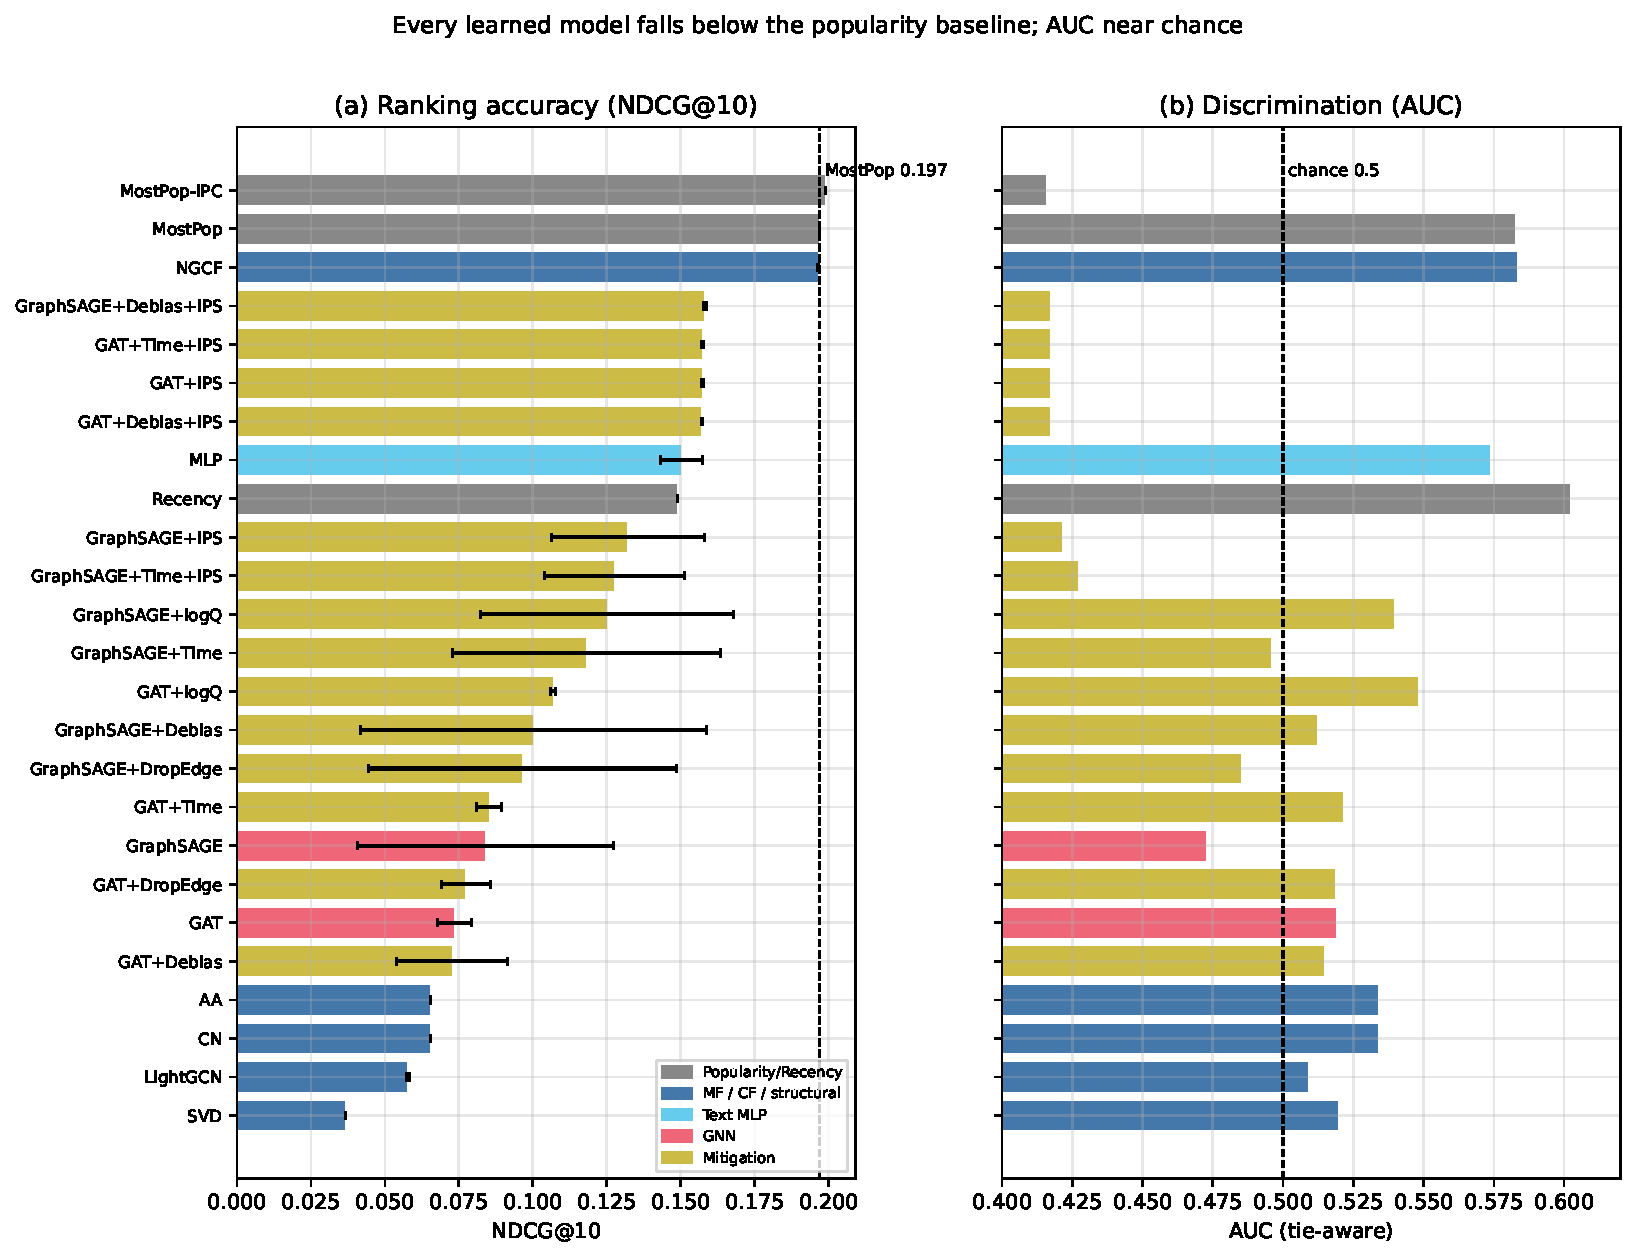
\includegraphics[width=\linewidth]{paper_figures/Figure_2}
\caption{Main results (temporal split). (a) NDCG@10 of all models, sorted; the dashed
line is the MostPop skyline (0.197). (b) Tie-aware AUC; the dashed line is chance
(0.5). Every learned model falls below the popularity baseline and discriminates near
chance.}
\label{fig:main}
\end{figure}

\subsection{Popularity Bias (RQ2)}
\label{sec:popbias}
Three diagnostics localize the failure to popularity bias (Table~\ref{tab:popbias},
Figure~\ref{fig:popbias}). (i) The Spearman $\rho$ between a model's candidate scores
and the candidates' training popularity is 1.0 for MostPop and 0.96 for NGCF
--- NGCF ranks almost exactly like a popularity counter, which is why its NDCG@10
(0.196) matches MostPop's. GAT has $\rho=-0.05$. (ii) A more-popular negative is
ranked above the true positive in 56.4\% of MostPop and 56.3\% of
NGCF queries, versus 28.4\% for GAT. (iii) A Mann--Whitney U test comparing
GAT's attention on edges to popular (top-5\%) hub companies versus non-hub companies
yields $p=1.0$: GAT does \emph{not} down-weight popular hubs. Stratifying GAT's
accuracy by company popularity shows it does worst on the popular head
(NDCG@10\,=\,0.016, torso 0.082) and best on the unpopular tail (0.370) --- the
opposite of a popularity-exploiting model, yet its absolute accuracy stays far below
MostPop because the head holds most positives, so the head-stratum score dominates
the aggregate (Figure~\ref{fig:stratified}).

\begin{table}[t]
\centering
\caption{Popularity-bias diagnostics (temporal).}
\label{tab:popbias}
\begin{tabular}{lcc}
\toprule
Model & Spearman $\rho$ (score, popularity) & Hard-neg inversion rate \\
\midrule
MostPop   & 1.00  & 56.4\% \\
NGCF      & 0.96  & 56.3\% \\
Recency   & 0.69  & 50.0\% \\
MLP       & 0.19  & 19.0\% \\
GraphSAGE & 0.07  & 51.5\% \\
SVD       & 0.02  & 2.4\%  \\
GAT       & $-0.05$ & 28.4\% \\
\bottomrule
\end{tabular}
\end{table}

\begin{figure}[t]
\centering
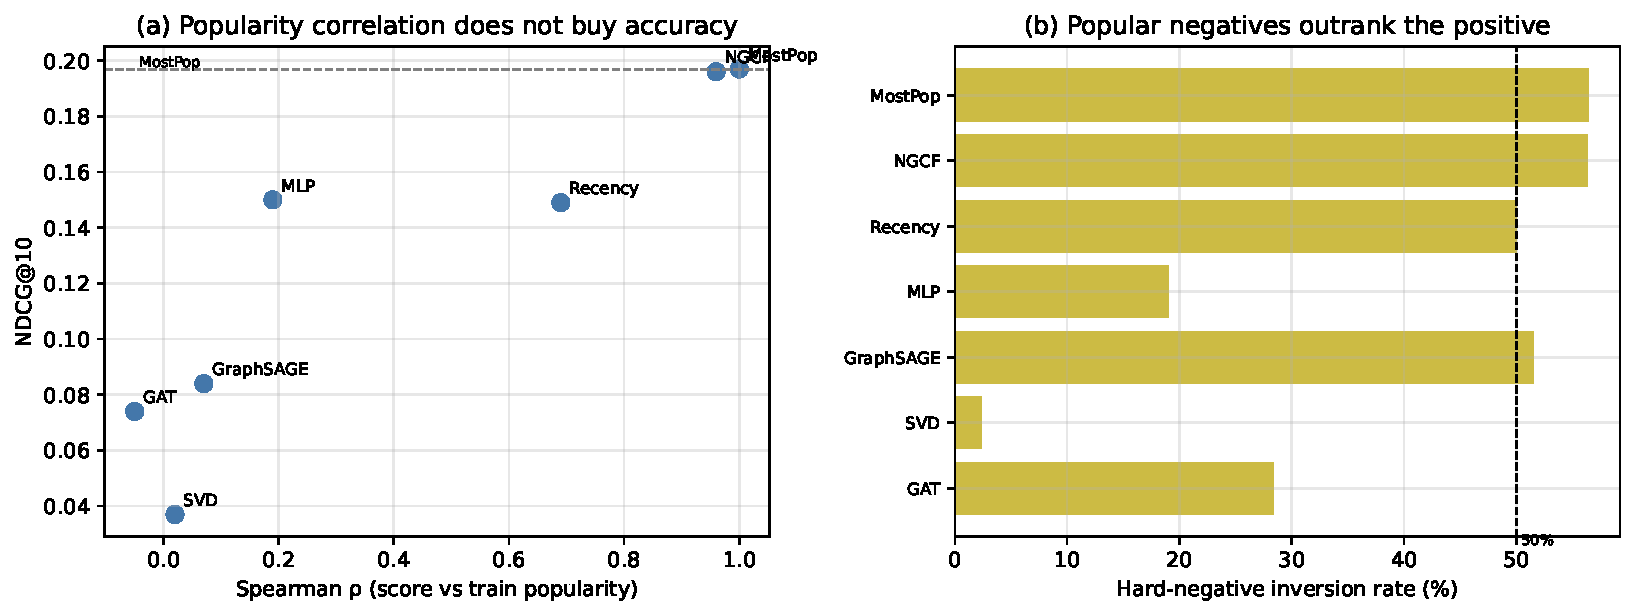
\includegraphics[width=\linewidth]{paper_figures/Figure_4}
\caption{Popularity bias. (a) Score--popularity Spearman $\rho$ vs.\ NDCG@10: high
correlation (MostPop, NGCF) coincides with high accuracy, but no learned model with
low correlation recovers it. (b) Hard-negative inversion rate: a more-popular negative
outranks the positive in 56\% of MostPop/NGCF queries.}
\label{fig:popbias}
\end{figure}

\begin{figure}[t]
\centering
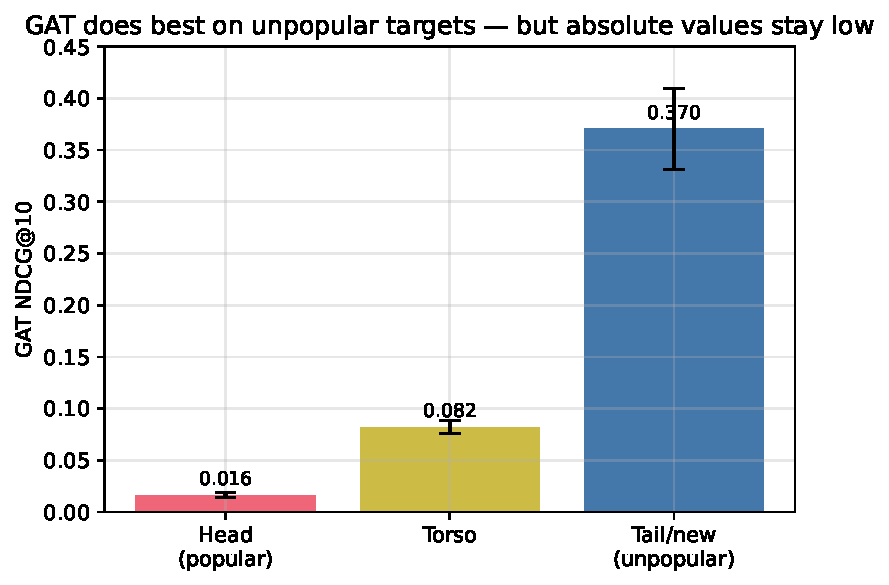
\includegraphics[width=0.7\linewidth]{paper_figures/Figure_5}
\caption{GAT NDCG@10 stratified by company popularity. GAT does best on the unpopular
tail and worst on the popular head, but absolute values stay far below MostPop.}
\label{fig:stratified}
\end{figure}

\subsection{Patent Cold-Start (RQ2)}
\label{sec:coldstart}
Under the temporal split, 91.7\% of test patents are unseen in training.
Decomposing accuracy by patent novelty matters most for SVD: on the new-patent subset
its NDCG@10 is 0.000 (its latent factor for an unseen patent is zero), whereas
on the seen-patent subset it reaches 0.439. Because new patents dominate, SVD's overall
score collapses to 0.037. The popularity baselines degrade gracefully (MostPop
new-patent 0.212 vs.\ seen 0.324) because a popular company remains a good guess
regardless of patent novelty; GAT is weak on both (0.022 / 0.021).
Figure~\ref{fig:coldstart} visualizes this.

\begin{figure}[t]
\centering
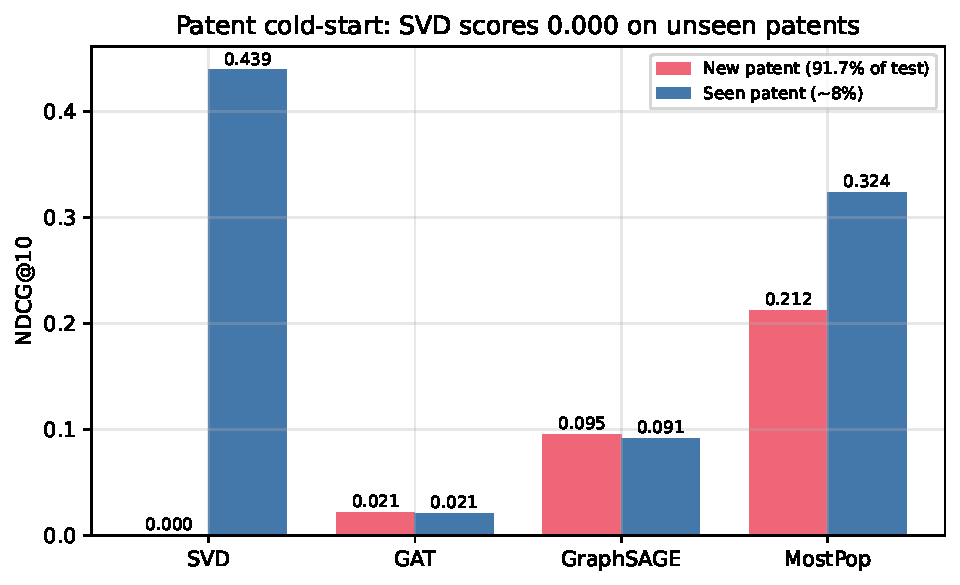
\includegraphics[width=0.75\linewidth]{paper_figures/Figure_6}
\caption{Patent cold-start. NDCG@10 on the new-patent (91.7\% of test) vs.\
seen-patent subsets. SVD scores 0.000 on new patents; the popularity baselines degrade
gracefully.}
\label{fig:coldstart}
\end{figure}

\subsection{Error-Source Decomposition (RQ2)}
\label{sec:error}
Attributing each failure to a cause (priority: popularity $>$ rare/new $>$ residual)
shows the backbones fail differently (Figure~\ref{fig:error}). For GraphSAGE,
98.8\% of failures are losses to a more-popular hard negative (0.1\% rare/new, 1.1\%
residual): it fails almost entirely through popularity. For GAT, the shares are 57.8\% /
8.3\% / 33.9\% --- popularity still dominates, but a third of GAT's errors are a
semantic residual, consistent with its near-zero popularity correlation. The two
backbones fail through different mechanisms.

\begin{figure}[t]
\centering
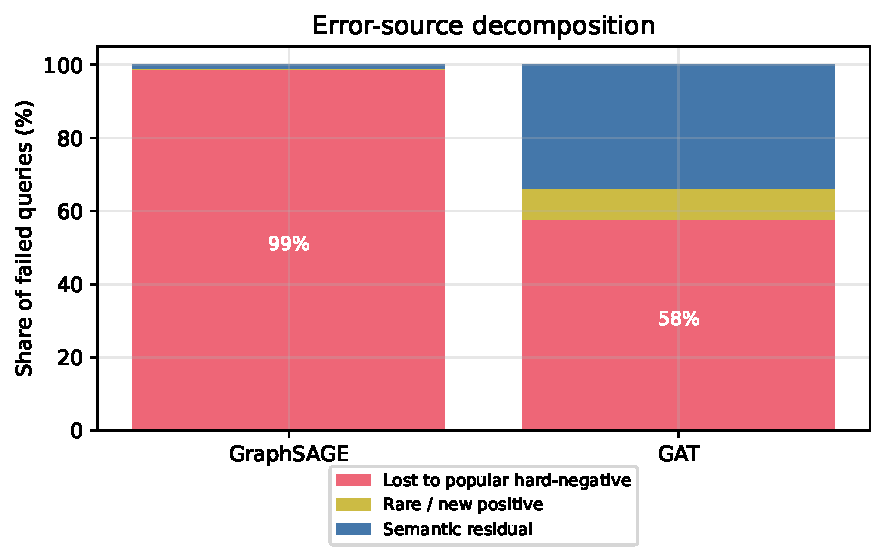
\includegraphics[width=0.6\linewidth]{paper_figures/Figure_7}
\caption{Error-source decomposition. Share of failed queries (rank $>$ 1) attributable
to each cause. GraphSAGE fails almost entirely through popularity; GAT spreads errors
across popularity and a semantic residual.}
\label{fig:error}
\end{figure}

\subsection{The Tie-Break Artifact}
\label{sec:tiebreak}
When many candidates receive identical scores --- the norm for cold-start models whose
representations are degenerate --- the tie-break rule determines the metric. Under a
strict greater-than rule the positive is placed ahead of every tied candidate \emph{by
construction}: because 91.7\% of test patents are cold and a fully-degenerate model
assigns every candidate the same score, such a model is ranked first on essentially
every cold query and appears near-perfect. In an earlier strict-rule evaluation this
inflated SVD (whose latent factor for an unseen patent is zero, leaving all candidates
tied) to NDCG@10 $\approx$ 0.95, and a fully-tied GraphSAGE+logQ to 1.00 by
construction. Replacing the strict rule with an \emph{average-rank} tie-break (a tie
contributes 0.5 to the positive's rank, so a fully-tied candidate set yields rank
$(n_{\mathrm{neg}}{+}1)/2$, i.e.\ chance) removes the artifact and returns these models
to their true ten-seed levels: SVD\,=\,0.037 and GraphSAGE+logQ\,=\,0.125 (and the
partially-degenerate GAT from $\approx$0.45 to 0.074). Figure~\ref{fig:tiebreak}
contrasts the rules. This is a generic pitfall for sampled-ranking
evaluation of cold-start link prediction.

\begin{figure}[t]
\centering
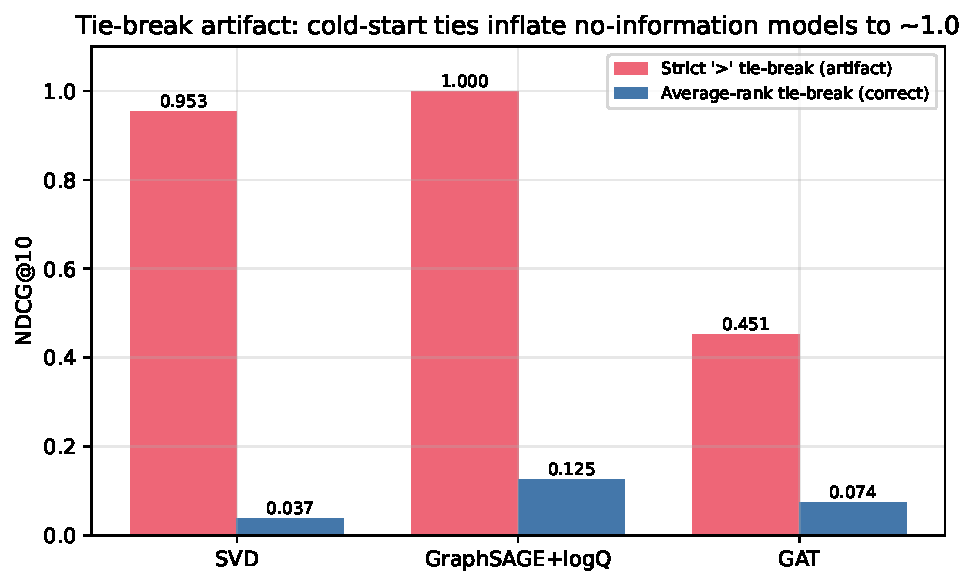
\includegraphics[width=0.65\linewidth]{paper_figures/Figure_3}
\caption{The tie-break artifact. Under a strict greater-than rule, degenerate
cold-start models are placed first on tied candidates and inflate toward perfect
scores; average-rank tie-breaking returns them to their true levels.}
\label{fig:tiebreak}
\end{figure}

\subsection{Robustness to the Sampled Metric}
\label{sec:sampled}
Two checks (both seed-0, since they are seed-invariant re-scorings of trained models)
confirm the verdict is not an artifact of the 100-negative sample. First, a
candidate-set-size sweep ($n_{\mathrm{neg}}\in\{50,100,200\}$) preserves the ordering:
MostPop NDCG@10\,=\,0.255 / 0.196 / 0.152 dominates GAT (0.104 / 0.082 / 0.069) at
every size. Second, an \emph{unsampled full-IPC-pool} ranking --- scoring each positive
against the entire eligible same-IPC pool (mean 900 candidates, capped at 1000; 78\% of
queries have pools exceeding 1000) --- preserves it too: MostPop\,=\,0.078,
GAT\,=\,0.058, SVD\,=\,0.028, GraphSAGE\,=\,0.008. Even against $\approx$9$\times$ more
candidates and with no sampling, no learned model beats MostPop \cite{krichene2020}.

\subsection{The Protocol Is Decisive: Temporal vs.\ Random (RQ1)}
\label{sec:rq1}
To quantify how much the protocol matters, we re-ran every model under a conventional
random 70/15/15 split (Table~\ref{tab:rq1}, Figure~\ref{fig:split}). A random split
lowers the patent cold-start rate from 91.7\% to 2.4\%, because patents are
scattered across train and test rather than held out by time. Under it,
matrix factorization becomes the single strongest method: SVD rises from
NDCG@10\,=\,0.037 (AUC 0.52) to 0.442 (AUC 0.830), comfortably exceeding
MostPop (0.219), reversing the temporal verdict. AUC inflates across the
board (MostPop $0.583\!\to\!0.667$; GAT $0.519\!\to\!0.650$). The mechanism is
straightforward: with only 2.4\% new patents, SVD's latent factors (useless on
truly-unseen patents --- its random-split new-patent NDCG@10 is still 0.0002) almost
always apply. A random-split evaluation would therefore have reported a clear
learned-model advantage; the realistic protocol, by exposing the cold-start regime the
random split conceals, reverses this outcome. This is the empirical core of RQ1 and the reason
near-perfect numbers in prior random-split patent recommenders \cite{kim2025} do not
contradict our diagnosis.

\begin{table}[t]
\centering
\caption{RQ1 contrast: NDCG@10 (AUC) under temporal vs.\ random splits.}
\label{tab:rq1}
\begin{tabular}{lcc}
\toprule
Model & Temporal & Random \\
\midrule
MostPop      & 0.197 (0.583) & 0.219 (0.667) \\
MostPop-IPC  & 0.199 (0.416) & 0.290 (0.604) \\
SVD          & 0.037 (0.520) & \textbf{0.442 (0.830)} \\
NGCF         & 0.196 (0.584) & 0.216 (0.663) \\
GAT          & 0.074 (0.519) & 0.165 (0.650) \\
\midrule
Patent cold-start rate & 91.7\% & 2.4\% \\
\bottomrule
\end{tabular}
\end{table}

\begin{figure}[t]
\centering
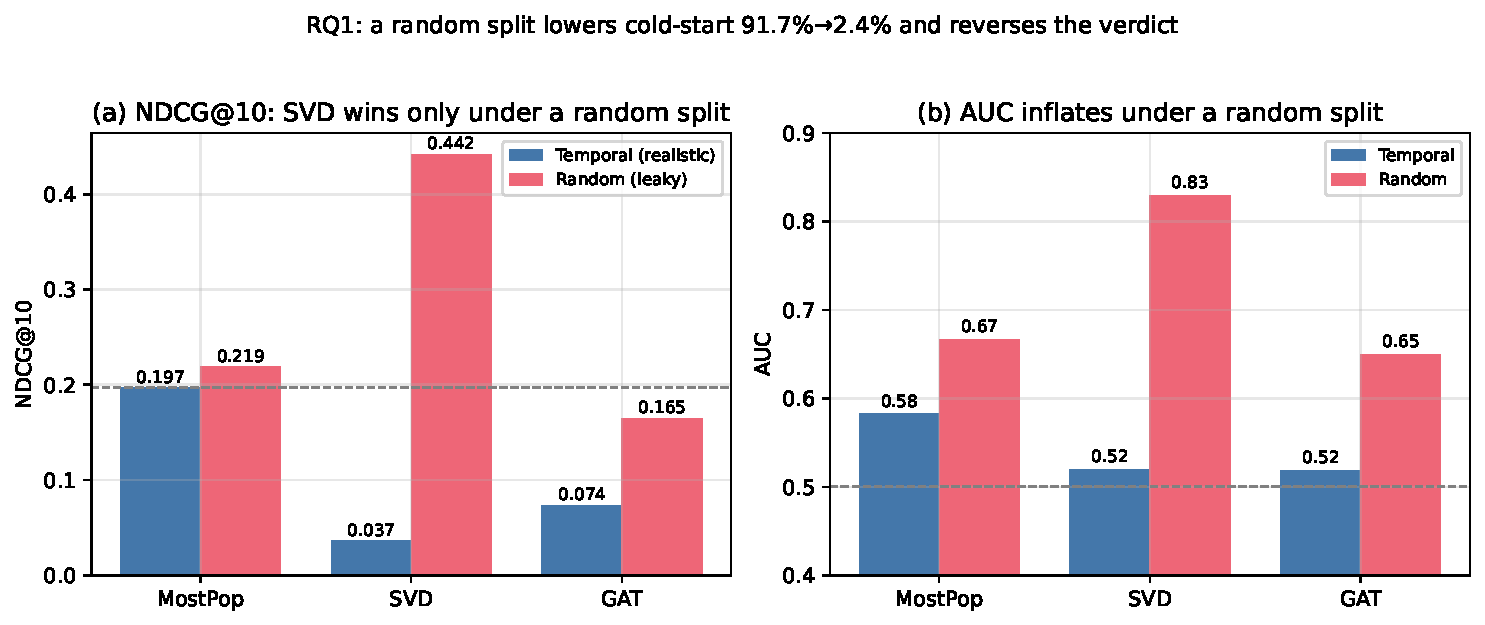
\includegraphics[width=\linewidth]{paper_figures/Figure_9}
\caption{RQ1: temporal vs.\ random split. A random split lowers the cold-start rate
(91.7\%$\to$2.4\%) and reverses the verdict --- (a) SVD becomes the best model by
NDCG@10, and (b) AUC inflates across the board.}
\label{fig:split}
\end{figure}

\subsection{Content company-feature ablation}
\label{sec:content}
A natural objection is that the GNNs underperform only because their company nodes
carry no content. We therefore replace the fixed-random company feature with the mean
frozen-SBERT embedding of each company's training-received patents --- a leakage-free
content representation (the 23.7\% of companies with no training transfer keep a random
fallback) --- and re-run the temporal protocol. Content company features do not lift
any learned model above the popularity baselines (Table~\ref{tab:content}): they leave
the bare GNNs essentially unchanged, and slightly lower (GraphSAGE
$0.084\!\to\!0.062$, GAT $0.074\!\to\!0.051$), and they sharply degrade the text MLP
($0.150\!\to\!0.032$, AUC $0.57\!\to\!0.40$), while the popularity skylines, SVD, and
the CF models are unaffected by construction (their scores do not use this feature).
Uninformative random company features are therefore not the explanation for the
diagnosis: even a leakage-free content representation of the company side does not
recover the transfer signal.

\begin{table}[t]
\centering
\caption{Content company-feature ablation (temporal split, NDCG@10 with AUC in
parentheses). Replacing the fixed-random company feature with the mean SBERT of each
company's training-received patents does not help the learned models. Rows whose scores
do not depend on the company feature (MostPop, NGCF, SVD, $\ldots$) are unchanged and
omitted.}
\label{tab:content}
\begin{tabular}{lcc}
\toprule
Model & Fixed-random feature & Content (mean-SBERT) feature \\
\midrule
Text MLP   & 0.150 (0.574) & 0.032 (0.399) \\
GraphSAGE  & 0.084 (0.473) & 0.062 (0.481) \\
GAT        & 0.074 (0.519) & 0.051 (0.504) \\
\midrule
MostPop (reference) & \multicolumn{2}{c}{0.197 (0.583)} \\
\bottomrule
\end{tabular}
\end{table}

\subsection{Rolling-origin robustness}
\label{sec:rolling}
To check that the diagnosis is not an artifact of the single 70/15/15 cutoff, we repeat
the evaluation under a rolling-origin (forward-chaining) protocol with three
expanding-window folds, each training on all transfers before a 5\% validation slice
and testing on a successive 10\% time slice (three seeds per fold). The verdict is
stable across all three folds (Table~\ref{tab:rolling}): the popularity skylines and
the popularity-equivalent NGCF lead at every cutoff (MostPop 0.200--0.210, MostPop-IPC
0.219--0.228), while every genuinely learned model stays below --- the strongest, a
text MLP, reaches 0.148--0.163, and the graph models remain far lower (GraphSAGE
0.076--0.113, GAT 0.050--0.066, SVD 0.042--0.060). The collapse of learned models below
the popularity baselines is therefore not specific to one split.

\begin{table}[t]
\centering
\caption{Rolling-origin robustness: NDCG@10 across three forward-chaining temporal
folds (three seeds each). No learned model surpasses the popularity baselines at any
cutoff.}
\label{tab:rolling}
\begin{tabular}{lccc}
\toprule
Model & Fold~1 (test 70--80\%) & Fold~2 (80--90\%) & Fold~3 (90--100\%) \\
\midrule
MostPop-IPC & 0.219 & 0.228 & 0.226 \\
MostPop     & 0.200 & 0.209 & 0.210 \\
NGCF        & 0.199 & 0.207 & 0.210 \\
MLP (text)  & 0.158 & 0.148 & 0.163 \\
GraphSAGE   & 0.113 & 0.092 & 0.076 \\
GAT         & 0.066 & 0.057 & 0.050 \\
SVD         & 0.047 & 0.060 & 0.042 \\
\bottomrule
\end{tabular}
\end{table}

%% ===========================================================================
\section{Mitigations (RQ3)}
\label{sec:mitigation}

We ask whether standard popularity-bias mitigations can lift a learned model above the
popularity baselines, applying each symmetrically to both GNN backbones:
popularity-debiased negative sampling, IPS / log-popularity
re-ranking, the logQ correction, DropEdge, a sinusoidal
transfer-edge time encoding, and the stacked combinations Debias+IPS and Time+IPS.
Concretely, popularity-debiased sampling draws hard negatives with probability
$P(c)\propto \mathrm{pop}_c^{\alpha}$ (exponent $\alpha$; $\alpha{=}0$ recovers uniform
same-IPC sampling); IPS / log-popularity re-ranking penalizes the inference score as
$\tilde{s}(p,c)=s(p,c)-\beta\log(\mathrm{pop}_c+1)$ (penalty $\beta$); and the logQ
correction subtracts the log negative-sampling probability from each candidate logit
during training, $s(p,c)\leftarrow s(p,c)-\log Q(c)$, debiasing the sampled-softmax
estimate. The gains are partial and unstable (Figure~\ref{fig:sweeps}).

\begin{itemize}
\item On GAT, two mitigations produce a small but statistically significant and
``honest'' (above-chance-AUC) gain: the logQ correction (NDCG@10 $0.074\!\to\!0.107$,
AUC 0.548) and the time encoding ($0.074\!\to\!0.085$, AUC 0.521), both at Wilcoxon
signed-rank Holm-adjusted $p=0.047$ --- yet both remain far below MostPop (0.197).
GraphSAGE+logQ reaches 0.125 but is \emph{not} significant after correction (high
cross-seed variance, Holm-adjusted $p\approx1.0$).
\item IPS re-ranking raises NDCG@10 the most --- GAT+IPS and GraphSAGE+Debias+IPS reach
$\approx$0.157--0.158 --- but at the cost of driving AUC to 0.417, below
chance: the penalty demotes popular candidates wholesale, helping the metric when the
positive is unpopular and hurting global discrimination. The $\beta$-sweep shows
NDCG@10 rising monotonically with the penalty (GAT $0.074\!\to\!0.157$) exactly as AUC
falls, confirming the trade-off is mechanical rather than a relevance gain.
\item Popularity-debiased sampling ($\alpha$) is noisy and non-monotone, never reaching
the baseline. DropEdge produces small, non-significant changes; the time encoding is
significant on GAT (above) but not on GraphSAGE.
\end{itemize}

\noindent No configuration in the grid reaches the popularity skyline; the mitigations
relocate error rather than remove it.

\begin{figure}[t]
\centering
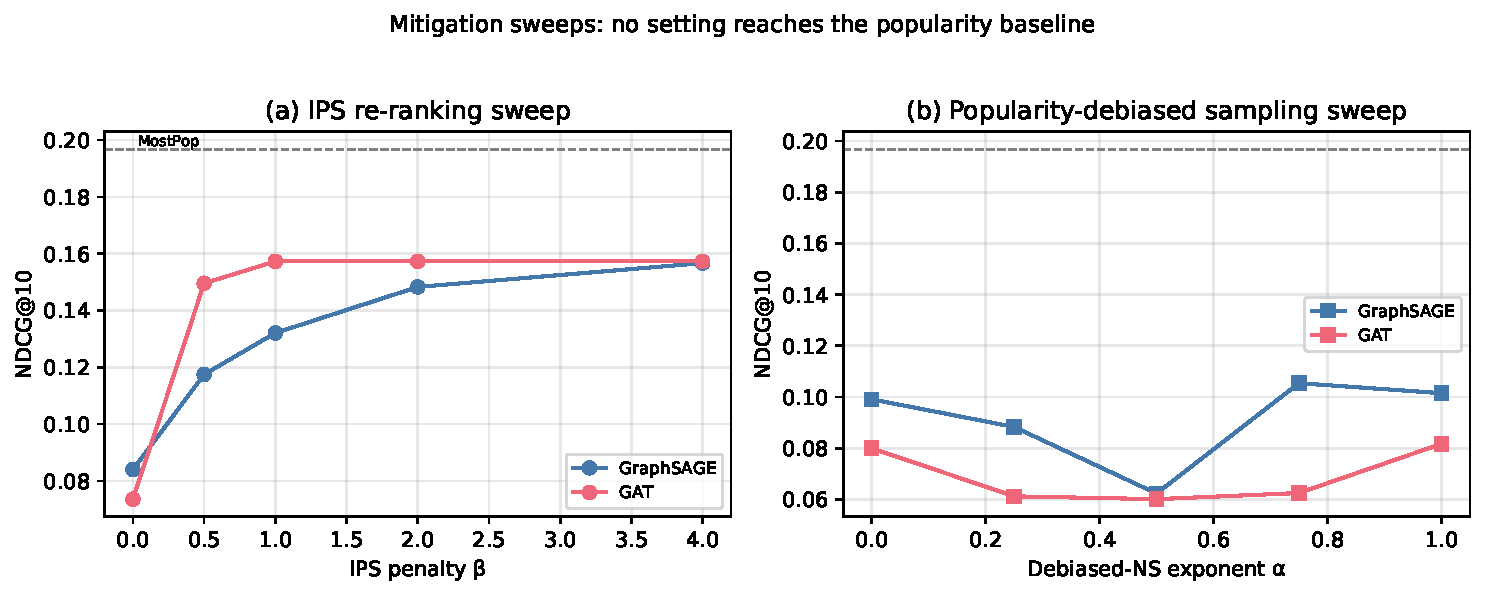
\includegraphics[width=\linewidth]{paper_figures/Figure_8}
\caption{Mitigation sweeps. (a) IPS penalty $\beta$ and (b) popularity-debiased
sampling exponent $\alpha$, per backbone. The dashed line is the MostPop skyline; no
setting reaches it, and IPS gains coincide with below-chance AUC.}
\label{fig:sweeps}
\end{figure}

%% ===========================================================================
\section{Limitations and Threats to Validity}
\label{sec:limitations}

\paragraph{Construct validity.} Our supervision is realized transfer, an
operationalization of latent demand; a model that perfectly predicted realized
transfers would recover the historical (and biased) matching process. We therefore
read the popularity-bias diagnosis partly as a property of the supervision signal.

\paragraph{Internal validity.} Transfer supervision is split strictly by registration
date and message-passed only on the training split; popularity/recency/time features
are train-only. Tie-breaking is average-rank, which we show is necessary. A residual
threat is that citation edges are not time-filtered, which we expect to be minor
relative to the transfer-edge leakage we control.

\paragraph{External validity.} All experiments use the Korean KIPRIS corpus. The
popularity-bias and cold-start regime are properties of this market's transfer record;
we cannot claim the same collapse would reproduce on a market with a different transfer
density or company-size distribution. The diagnosis is established for one jurisdiction
and is a hypothesis elsewhere.

\paragraph{Statistical-conclusion validity.} Ten seeds with Wilcoxon signed-rank +
Holm--Bonferroni and bootstrap CIs over queries; we report effect sizes alongside
adjusted $p$-values so a significant but negligible gain (e.g.\ logQ's $+0.033$ NDCG@10
on GAT, still below MostPop) is not over-read. The random-ranking floors are
NDCG@10 $\approx$ 0.045 and AUC\,=\,0.5; AUC near 0.5 with above-floor NDCG is not a
contradiction but the signature of a popularity prior.

\paragraph{Temporal cutoff.} Our main results use a single 70/15/15 temporal split. We
verify that the diagnosis is not specific to this cutoff with a three-fold
rolling-origin evaluation (\S\ref{sec:rolling}), in which no learned model beats the
popularity baselines at any cutoff, and with the controlled random-split contrast
(\S\ref{sec:rq1}), which confirms that the realistic protocol is what exposes the
failure. A finer-grained or longer rolling horizon remains possible future work.

\paragraph{Future work.} Replication on USPTO/EPO records and public link-prediction
benchmarks; rolling-origin evaluation; content-aware company representations and
cold-start-specific architectures; and treatment of the realized-transfer/latent-demand
gap via exposure modeling.

\paragraph{Generalizability.} The quantitative verdict --- the magnitude of the
cold-start rate, the size of the popularity-baseline gap, and the temporal-vs-random
reversal --- is specific to the KIPRIS transfer record and its company-size
distribution, and we do not claim the same ordering reproduces on markets with
different transfer density. What we expect to generalize is methodological: the
protocol (temporal split, same-class hard negatives, cold-start accounting,
average-rank tie-break), the bias and cold-start diagnostics, and the
strict-tie-break artifact are dataset-agnostic and apply to any sampled-ranking
evaluation of cold-start-heavy link prediction.

%% ===========================================================================
\section{Conclusion}
\label{sec:conclusion}

We examined patent technology-transfer demand prediction as link prediction over a
heterogeneous patent--citation--transfer graph, and asked whether learned models
recover useful demand signal under a realistic protocol. Across heterogeneous GNNs
(GraphSAGE, GAT), CF recommenders (LightGCN, NGCF), matrix factorization (SVD),
structural heuristics (Common Neighbors, Adamic--Adar), and a text MLP, no learned
model surpasses a simple popularity baseline when the evaluation uses a temporal split,
same-IPC hard negatives, and an average-rank tie-break. The strongest configurations
are not learned: MostPop-IPC (0.199), MostPop (0.197), and a popularity-equivalent NGCF
(0.196); the strongest learned model, a text MLP, reaches only 0.150, and every
graph-based model is lower (GraphSAGE+logQ 0.125, GAT+logQ 0.107), with AUC near chance
(0.42--0.60). Two compounding causes account for this: popularity bias (98.8\% of
GraphSAGE and 57.8\% of GAT errors are losses to a more-popular hard negative; $\rho$ up
to 1.0) and extreme patent cold-start (91.7\% unseen; SVD 0.000 on new patents). The
mitigations we evaluate yield only partial, unstable gains: logQ significantly improves
GAT ($0.074\!\to\!0.107$) yet stays below MostPop, and IPS re-ranking raises NDCG@10 to
$\approx$0.157 only by driving AUC to 0.417. We additionally document an evaluation
artifact --- a strict tie-break inflates degenerate cold-start models to near-perfect
scores ($\approx$0.95--1.00), corrected to 0.037 and 0.125 by average-rank --- and show
the diagnosis survives an unsampled full-pool metric. Finally, the protocol is
decisive: under a random split the cold-start rate falls to 2.4\% and matrix
factorization becomes the single best method (0.442, AUC 0.830), reversing
the temporal verdict. Our aim has been not a winning model but an evaluation protocol
and a diagnosis --- with reusable bias-diagnostic tools --- to discipline future work on
patent technology-transfer prediction and on cold-start-heavy link prediction more
broadly.

\paragraph{Implications for research and practice.} For \emph{research},
the results argue for reporting patent-recommendation and technology-transfer
results under temporal splits with same-class hard negatives and explicit
cold-start accounting, and for treating a popularity baseline and an AUC sanity
check as mandatory reference points; near-perfect random-split numbers should be
read as upper bounds, not as deployment estimates. For \emph{practice},
technology-transfer intermediaries should not expect a learned ranker to
outperform a simple popularity or recency heuristic on genuinely new patents
under this market's data, and a popularity prior is a defensible, low-cost
operational default; closing the gap will require content-aware company
representations and exposure-aware supervision rather than a change of graph
architecture alone.

%% ===========================================================================
\section*{Data availability}
The patent data were obtained from the Korea Intellectual Property Rights Information
Service (KIPRIS) through its paid API (KIPRIS Plus, \url{https://plus.kipris.or.kr})
and were subsequently cleaned and processed by the authors. Because redistribution of
these data is restricted by the KIPRIS terms of use, the processed dataset is not
deposited in a public repository; it is instead available from the authors by email
upon reasonable request, subject to those terms. The preprocessing and
evaluation code, the experiment scripts, and a script to regenerate the frozen SBERT
embeddings from patent text are released, so that all tables and figures can be
reproduced once the KIPRIS exports are obtained.

%% ===========================================================================
\section*{Declaration of generative AI and AI-assisted technologies in the manuscript preparation process}
During the preparation of this work the authors used Claude (Anthropic) in order to
improve the language, grammar, and readability of the manuscript. After using this
tool, the authors reviewed and edited the content as needed and take full
responsibility for the content of the published article. The figures are data
visualizations generated by the authors' own analysis code directly from the
experimental results, without generative AI.

%% ===========================================================================
\bibliographystyle{elsarticle-num}
%% Inline numbered bibliography (no .bib needed). For final submission this block may
%% be replaced by \bibliography{refs} with a BibTeX database.

\begin{thebibliography}{99}

\bibitem{kimgeum2020}
Kim, J., Geum, Y., 2020. Predicting patent transactions using patent-based machine learning techniques. IEEE Access 8, 188833--188843.

\bibitem{lee2016}
Lee, C., Lee, G., Yoon, B., 2016. Identifying product opportunities using collaborative filtering-based patent analysis. Computers \& Industrial Engineering 99, 247--257.

\bibitem{rhee2026}
Rhee, Kim, Lee, Park, Sung, 2026. Predicting patent transaction cycle using neural hazard model: evidence from technology transactions between companies in South Korea. Scientometrics 131(4), 2549--2583.

\bibitem{parkyoon2017}
Park, I., Yoon, B., 2017. Application technology opportunity discovery from technology portfolios: Use of patent classification and collaborative filtering. Technological Forecasting and Social Change 118, 170--183.

\bibitem{abbasiantaeb2025}
Abbasiantaeb, Z., Verberne, S., Wang, S., 2025. Tracing science-technology-linkages: A machine learning pipeline for extracting and matching patent in-text references to scientific publications. Information Processing \& Management 62, 104264.

\bibitem{hamilton2017}
Hamilton, W.L., Ying, R., Leskovec, J., 2017. Inductive representation learning on large graphs (GraphSAGE), in: Advances in Neural Information Processing Systems (NeurIPS 2017). arXiv:1706.02216.

\bibitem{velickovic2018}
Veli\v{c}kovi\'{c}, P., Cucurull, G., Casanova, A., Romero, A., Li\`{o}, P., Bengio, Y., 2018. Graph attention networks, in: International Conference on Learning Representations (ICLR 2018). arXiv:1710.10903.

\bibitem{brody2022}
Brody, S., Alon, U., Yahav, E., 2022. How attentive are graph attention networks? (GATv2), in: International Conference on Learning Representations (ICLR 2022). arXiv:2105.14491.

\bibitem{wang2019}
Wang, X., He, X., Wang, M., Feng, F., Chua, T.-S., 2019. Neural graph collaborative filtering (NGCF), in: Proceedings of SIGIR 2019. arXiv:1905.08108.

\bibitem{he2020}
He, X., Deng, K., Wang, X., Li, Y., Zhang, Y., Wang, M., 2020. LightGCN: Simplifying and powering graph convolution network for recommendation, in: Proceedings of SIGIR 2020. arXiv:2002.02126.

\bibitem{rendle2009}
Rendle, S., Freudenthaler, C., Gantner, Z., Schmidt-Thieme, L., 2009. BPR: Bayesian personalized ranking from implicit feedback, in: Proceedings of UAI 2009. arXiv:1205.2618.

\bibitem{reimers2019}
Reimers, N., Gurevych, I., 2019. Sentence-BERT: Sentence embeddings using Siamese BERT-networks, in: Proceedings of EMNLP 2019. arXiv:1908.10084.

\bibitem{reimers2020}
Reimers, N., Gurevych, I., 2020. Making monolingual sentence embeddings multilingual using knowledge distillation, in: Proceedings of EMNLP 2020.

\bibitem{krestel2021}
Krestel, R., Chikkamath, R., Hewel, C., Risch, J., 2021. A survey on deep learning for patent analysis. World Patent Information.

\bibitem{choi2019}
Choi, Lee, Park, Choi, 2019. Deep patent landscaping model using Transformer and graph embedding. arXiv:1903.05823 (Expert Systems with Applications 2022).

\bibitem{chendeng2023}
Chen, Deng, 2023. Interpretable patent recommendation with knowledge graph and deep learning. Scientific Reports 13, 2586.

\bibitem{liu2024}
Liu, Zhang, Deng, Ma, Fan, 2024. A deep learning method for recommending university patents to industrial clusters by common technological needs mining. Scientometrics.

\bibitem{kim2025}
Kim, M.-S., Jang, Y.-J., Sung, T.-E., 2025. Graph-based technology recommendation system using GAT-NGCF. Expert Systems with Applications 280.

\bibitem{meng2020}
Meng, Z., McCreadie, R., Macdonald, C., Ounis, I., 2020. Exploring data splitting strategies for the evaluation of recommendation models, in: Proceedings of RecSys 2020. arXiv:2007.13237.

\bibitem{krichene2020}
Krichene, W., Rendle, S., 2020. On sampled metrics for item recommendation, in: Proceedings of KDD 2020 (CACM 2022).

\bibitem{abdollahpouri2019}
Abdollahpouri, H., Burke, R., Mobasher, B., 2019. Managing popularity bias in recommender systems with personalized re-ranking, in: Proceedings of FLAIRS 2019. arXiv:1901.07555.

\bibitem{steck2018}
Steck, H., 2018. Calibrated recommendations, in: Proceedings of RecSys 2018.

\bibitem{zhu2021}
Zhu, Z., He, Y., Zhao, X., Zhang, Y., Wang, J., Caverlee, J., 2021. Popularity-opportunity bias in collaborative filtering, in: Proceedings of WSDM 2021.

\bibitem{boratto2021}
Boratto, L., Fenu, G., Marras, M., 2021. Connecting user and item perspectives in popularity debiasing for collaborative recommendation. Information Processing \& Management 58(1), 102387.

\bibitem{deldjoo2021}
Deldjoo, Y., Bellog\'{\i}n, A., Di Noia, T., 2021. Explaining recommender systems fairness and accuracy through the lens of data characteristics. Information Processing \& Management 58(5), 102662.

\bibitem{boratto2023}
Boratto, L., Fenu, G., Marras, M., Medda, G., 2023. Practical perspectives of consumer fairness in recommendation. Information Processing \& Management 60(2), 103208.

\bibitem{dacrema2019}
Ferrari Dacrema, M., Cremonesi, P., Jannach, D., 2019. Are we really making much progress? A worrying analysis of recent neural recommendation approaches, in: Proceedings of RecSys 2019. arXiv:1907.06902.

\bibitem{li2023}
Li, J., Shomer, H., Mao, H., Zeng, S., Ma, Y., Shah, N., Tang, J., Yin, D., 2023. Evaluating graph neural networks for link prediction: Current pitfalls and new benchmarking (HeaRT), in: Advances in Neural Information Processing Systems (NeurIPS 2023 Datasets and Benchmarks). arXiv:2306.10453.

\bibitem{hidasi2023}
Hidasi, B., Czapp, \'{A}.T., 2023. Widespread flaws in offline evaluation of recommender systems, in: Proceedings of RecSys 2023. arXiv:2307.14951.

\bibitem{schnabel2016}
Schnabel, T., Swaminathan, A., Singh, A., Chandak, N., Joachims, T., 2016. Recommendations as treatments: Debiasing learning and evaluation (IPS), in: Proceedings of ICML 2016. arXiv:1602.05352.

\bibitem{saito2020}
Saito, Y., Yaginuma, S., Nishino, Y., Sakata, H., Nakata, K., 2020. Unbiased recommender learning from missing-not-at-random implicit feedback, in: Proceedings of WSDM 2020. arXiv:1909.03601.

\bibitem{yi2019}
Yi, X., et al., 2019. Sampling-bias-corrected neural modeling for large corpus item recommendations (logQ), in: Proceedings of RecSys 2019.

\bibitem{rong2020}
Rong, Y., Huang, W., Xu, T., Huang, J., 2020. DropEdge: Towards deep graph convolutional networks on node classification, in: International Conference on Learning Representations (ICLR 2020). arXiv:1907.10903.

\bibitem{schlichtkrull2018}
Schlichtkrull, M., Kipf, T.N., Bloem, P., van den Berg, R., Titov, I., Welling, M., 2018. Modeling relational data with graph convolutional networks (R-GCN), in: Proceedings of ESWC 2018. arXiv:1703.06103.

\bibitem{hu2020hgt}
Hu, Z., Dong, Y., Wang, K., Sun, Y., 2020. Heterogeneous graph transformer (HGT), in: Proceedings of WWW 2020. arXiv:2003.01332.

\bibitem{zhang2018}
Zhang, M., Chen, Y., 2018. Link prediction based on graph neural networks (SEAL), in: Advances in Neural Information Processing Systems (NeurIPS 2018). arXiv:1802.09691.

\bibitem{erdi2013}
\'{E}rdi, P., et al., 2013. Prediction of emerging technologies based on analysis of the U.S. patent citation network. Scientometrics 95(1). arXiv:1206.3933.

\bibitem{rendle2019}
Rendle, S., Zhang, L., Koren, Y., 2019. On the difficulty of evaluating baselines: A study on recommender systems. arXiv:1905.01395.

\bibitem{canamares2020}
Ca\~{n}amares, R., Castells, P., 2020. On target item sampling in offline recommender system evaluation, in: Proceedings of RecSys 2020.

\bibitem{ihemelandu2023}
Ihemelandu, N., Ekstrand, M.D., 2023. Candidate set sampling for evaluating top-N recommendation. arXiv:2309.11723.

\bibitem{ji2023}
Ji, Y., Sun, A., Zhang, J., Li, C., 2023. A critical study on data leakage in recommender system offline evaluation. ACM Transactions on Information Systems 41(3). arXiv:2010.11060.

\bibitem{volkovs2017}
Volkovs, M., Yu, G., Poutanen, T., 2017. DropoutNet: Addressing cold start in recommender systems, in: Advances in Neural Information Processing Systems (NeurIPS 2017).

\end{thebibliography}

\end{document}
